
\section{mitemset.rb - Enumerate Frequent Itemsets \label{sect:mitemset}}

This program enumerates frequent itemsets from the transaction data using LCM (Linear time Closed itemset Miner) as the core algorithm for itemset enumeration\cite{Uno2004,UnoWeb}. 

This command have the following features: 
\begin{itemize}
 \item Enumerate "maximal itemsets" that is not contained in other itemsets. 
 \item Enumerate "emerging itemsets" that contains the maximal itemsets with similar features.
 \item Use item taxonomy for hierarchical classification. 
 \item By specifying classification class, patterns with specific features particular to the class is enumerated (emerging patterns).
Supports 3 or more classes. 
\end{itemize}


The different types of input data are shown in Table \ref{tbl:key},\ref{tbl:tra},\ref{tbl:matrix}, 
however, note that this command can only process key-based data (Table \ref{tbl:key}).
The \verb|mtra| and \verb|mtraflg| in MCMD package can be used to convert other data types to key-based data beforehand. 


Table \ref{tbl:key} contains records with the same \verb|key| field, on the other hand, Table \ref{tbl:tra},\ref{tbl:matrix} display transaction containing relevant items in one record. 

In case of supermarket, consider  items as merchandise purchased for each transaction receipt. 



\begin{table}[htbp]
\begin{center}
\begin{tabular}{ccc}

\begin{minipage}{0.3\hsize}
\begin{center}
\caption{Key based data\label{tbl:key}}
{\small
\begin{tabular}{cc}
\hline
key&item \\
\hline
T1&C \\
T1&E \\
T2&D \\
T2&E \\
T2&F \\
:&: \\ \hline
\end{tabular} 
}
\end{center}
\end{minipage}

\begin{minipage}{0.3\hsize}
\begin{center}
\caption{Tra type data\label{tbl:tra}}
{\small
\begin{tabular}{ll}
\hline
id&item \\
\hline
T1&C E \\
T2&D E F \\
T3&A B D F \\
T4&B D F \\
T5&A B D E \\
T6&A B D E F \\
\hline
\end{tabular} 
}
\end{center}
\end{minipage}

\begin{minipage}{0.3\hsize}
\begin{center}
\caption{Row type data\label{tbl:matrix}}
{\small
\begin{tabular}{ccccccc}
\hline
id&A&B&C&D&E&F \\
\hline
T1& & &1& &1& \\
T2& & & &1&1&1\\
T3&1&1& &1& &1\\
T4& &1& &1& &1\\
T5&1&1& &1&1& \\
T6&1&1& &1&1&1\\
\hline
\end{tabular} 
}
\end{center}
\end{minipage}

\end{tabular} 
\end{center}
\end{table} 



\subsubsection*{Frequent itemset}
A Frequent itemset refers to a set of items of which the frequency (known as support) is more than or equal to the minimum support provided by the user.

Using the input data in Table \ref{tbl:tra} as an example, when the minimum support is set as 3, itemset \{B,D,F\} appeared in T3,T5,T6 and is considered as frequent. However, itemset \{B,D,E\} only appeared in T5,T6 and it is not considered.

There are a total of 13 frequent itemsets meeting the minimum support of 3 including
\{A\},
\{A,B\},
\{A,B,D\},
\{A,D\},
\{B\},
\{B,D\},
\{B,D,F\},
\{B,F\},
\{D\},
\{D,E\},
\{D,F\},
\{E\},
\{F\}.

Since a large number of frequent itemset candidates are enumerated, two enumeration methods namely maximum itemset and closed itemset can be used to select representative itemsets in the output. 

\subsubsection*{Maximal itemset}
A maximal itemset is a frequent itemset which is included in no other frequent itemsets.  
In Table \ref{tbl:tra}, three itemsets \{A,B,D\},\{B,D,F\},\{D,E\} are not included in any other itemsets. Therefore, it is referred to as maximal item set.
Other itemsets are not maximal since they are included in more than 3 maximal itemsets.

\subsubsection*{Closed itemset}
Select any two frequent itemsets, if they appear in the same transaction, they are considered as the same group of itemset.
By grouping all frequent itemsets, if there are no superset that has the same support as the frequent itemset, the itemset is referred to as closed set.
For example, \{A\},\{A,B\},\{A,D\},\{A,B,D\} appear in transactions T3,T5,T6 and they are classified as the same group.

\{A,B,D\} is returned as closed itemset with maximum frequency, and itemsets \{A\},\{A,B\},\{A,D\} are not included in output. 

Table \ref{tbl:close}  a total of seven patterns are enumerated from closed itemsets. The number of itemsets enumerated are reduced significantly as closed itemsets only enumerate representative itemsets. 
%ただし、データによっては、飽和集合を列挙したとしても全く列挙件数が減少しない
%ことも有りうる。

\begin{table}[htbp]
\begin{center}

\caption{Closed itemset\label{tbl:close}}
{\small
\begin{tabular}{lll}
\hline
Closed set&Transaction&Group \\
\hline
\{A,B,D\} & T3,T5,T6       & \{A\},\{A,B\},\{A,D\},\{A,B,D\} \\
\{B,D\}   & T3,T4,T5,T6    & \{B\},\{B,D\}  \\
\{B,D,F\} & T3,T4,T6       & \{B,F\},\{B,D,F\} \\
\{D\}     & T2,T3,T4,T5,T6 & \{D\} \\
\{D,E\}   & T2,T5,T6       & \{D,E\}    \\
\{D,F\}   & T2,T3,T4,T6    & \{F\},\{D,F\} \\
\{E\}     & T1,T2,T5,T6    & \{E\} \\ \hline
\end{tabular} 
}

\end{center}
\end{table} 



\subsubsection*{Emerging patterns}
Emerging patterns enumerate particular patterns (frequent itemset) from pre-defined class that it is frequent for one data class and not frequent for another class, and whose support changes significantly.
The feature characteristics in one class is not frequent in other classes. 
For instance, it can be used to identify different items purchased by men or women in a supermarket.

Please refer to \hyperref[sect:ep]{Appendix 1} for more detailed definition of emerging pattern. 
The class data shown in \ref{tbl:class} is created by combining the class item to the transaction data.
Rows with the same transaction key will be assigned with the same class value. 
 
\begin{table}[htbp]
\begin{center}
\caption{Key-based data\label{tbl:class}}
{\small
\begin{tabular}{ccc}
\hline
key&item&class \\
\hline
T1&C&pos \\
T1&E&pos \\
T2&D&neg \\
T2&E&neg \\
T2&F&neg \\
:&: \\ \hline
\end{tabular}
}
\end{center}
\end{table}

\subsubsection*{Hierarchical classification}
Hierarchical classification can be designated for individual items. 
For example, in a supermarket, an item "Milk 500ml" is classified as "Milk", subsequently, "Milk" is classified under "Milk product", and "Milk product" is classified as "Food".
By using hierarchical classification, it is possible to find out whether "Milk 500ml" and "Fruit" are frequently purchased at the same time.
Note that the current version only allows for one hierarchy.

The internal processing can be simplified as follows. Given the corresponding relationship between item and classification (Table \ref{tbl:map}), corresponding classifications are combined with certain items in the input data (Table \ref{tbl:org}) as shown in Table \ref{tbl:add}.  Alternatively, the classifications substitute the corresponding itemsets in the input data as shown in Table \ref{tbl:rep}.  

\begin{table}[htbp]
\begin{center}
\begin{tabular}{ccc}

\begin{minipage}{0.25\hsize}
\begin{center}
\caption{Original data\label{tbl:org}}
{\small
\begin{tabular}{ll}
\hline
id&item \\
\hline
T1&C E \\
T2&D E F \\
T3&A B D F \\
T4&B D F \\
T5&A B D E \\
T6&A B D E F \\
\hline
\end{tabular} 
}
\end{center}
\end{minipage}

\begin{minipage}{0.25\hsize}
\begin{center}
\caption{Item-classification mapping table\label{tbl:map}}
{\small
\begin{tabular}{cc}
\hline
item&taxonomy \\
\hline
A&X \\
B&X \\
C&Y \\
D&Z \\
E&Z \\
F&Z \\ \hline
\end{tabular} 
}
\end{center}
\end{minipage}

\begin{minipage}{0.25\hsize}
\begin{center}
\caption{Data combined with classification\label{tbl:add}}
{\small
\begin{tabular}{ll}
\hline
id&item \\
\hline
T1&C E Y Z\\
T2&D E F Z \\
T3&A B D F X Z\\
T4&B D F Y Z\\
T5&A B D E X Z\\
T6&A B D E F X Z\\
\hline
\end{tabular} 
}
\end{center}
\end{minipage}

\begin{minipage}{0.25\hsize}
\begin{center}
\caption{Data substituted with classification\label{tbl:rep}}
{\small
\begin{tabular}{ll}
\hline
id&item \\
\hline
T1&Y Z\\
T2&Z \\
T3&X Z\\
T4&Y Z\\
T5&X Z\\
T6&X Z\\
\hline
\end{tabular} 
}
\end{center}
\end{minipage}


\end{tabular} 
\end{center}
\end{table} 


\subsubsection{Output}
This command returns two main output data, the first is the enumerated pattern data (\verb|patterns.csv|), the other contains information about the transaction for the corresponding pattern (\verb|tid_pats.csv|). 
CSV columns in output pattern data are different for emerging pattern.
The sample is shown in Table \ref{tbl:pat} to Table \ref{tbl:ep_pat}. 

\begin{table}[htbp]
\begin{center}
\begin{tabular}{cc}

\begin{minipage}{0.6\hsize}
\begin{center}
\caption{Example of patterns.csv data\label{tbl:pat}. The column pid contains the unique ID  which differentiates each pattern, size refers to the number of items consists in the pattern,  count refers to the number of transactions the pattern appears, 
total refers to the number of all transactions. Support of probability of occurrence is calculated by count/total. Lift compares the expected probability with actual probability to measure the performance of target model. 
The last column contains pattern of itemset, the items are delimited by space.}
{\small
\begin{tabular}{crrrrrl}
\hline
pid&size&count&total&support&lift&pattern\\
\hline
 1&1&5&6&0.8333333333&1&D\\
 7&2&4&6&0.6666666667&1.2&D F\\
 6&1&4&6&0.6666666667&1&F\\
 4&1&4&6&0.6666666667&1&E\\
 2&1&4&6&0.6666666667&1&B\\
 3&2&4&6&0.6666666667&1.2&B D\\
 8&2&3&6&0.5&1.125&B F\\
 13&2&3&6&0.5&1.2&A D\\
\hline
\end{tabular} 
}
\\
{\small
Value of lift lift($I$) for itemset $I=\{i_1,i_2,\cdots,i_n\}$ is defined as follows.
lift($I$)$=\frac{\Pr(I)}{\prod_{k=1}^n \Pr(i_k)}$
}
\end{center}
\end{minipage}
\begin{minipage}{0.3\hsize}
\begin{center}
\caption{Contents of tidpats.csv\label{tbl:tid_pats}. Tid is the transaction ID, which corresponds to the column in the input data defined at tid= parameter. 
The ID of each pattern for each transaction is identified by pid. 
}
{\small
\begin{tabular}{cr}
\hline
tid&pid \\
\hline
 T1&4\\
 T2&1\\
 T2&4\\
 T2&7\\
 T2&6\\
 T2&5\\
 T3&10\\
 T3&6\\
\hline
\end{tabular} 
}
\end{center}
\end{minipage}

\end{tabular} 
\end{center}
\end{table} 

\begin{table}[htbp]
\begin{center}
\caption{Example of emerging patterns in patterns.csv\label{tbl:ep_pat}.
The class field indicates the target class based on the characteristics shown in emerging patterns. Attributes pid, pattern, size, total shown in Table \ref{tbl:pat} are defined in the previous table. 
Pos refers to the number of target class appeared in the transaction, neg is the number of other classes in the transaction. 
The total transaction numbers of target and and non target classes are indicated in posTotal and negTotal respectively. 
Support is the probability of occurrence, calculated by pos/posTotal.
The change is represented by growthRate, calculated by support/(neg/negTotal). 
The result is shown as inf when the denominator is 0.
As this value increases, the key feature for target class emerges. Posterior probability of the target class is represented by postProb, as with growthRate, as the value grow larger, it shows the key feature for the target class. Detailed definition is illustrated in  \hyperref[sect:ep]{Appendix 1} in mitemset.rb command manual. 
}
\vspace{1em}
{\small
\begin{tabular}{cclrrrrrrrrr}
\hline
class&pid&pattern&size&pos&neg&posTotal&negTotal&total&support&growthRate&postProb\\
\hline
 cls2&13&A E&2&2&0&2&4&6&1&inf&1\\
 cls2&15&A B E&3&2&0&2&4&6&1&inf&1\\
 cls2&10&A B D E&4&2&0&2&4&6&1&inf&1\\
 cls2&14&B E&2&2&0&2&4&6&1&inf&1\\
 cls2&17&A D E&3&2&0&2&4&6&1&inf&1\\
 cls2&18&B D E&3&2&0&2&4&6&1&inf&1\\
 cls2&12&A B D&3&2&1&2&4&6&1&4&0.6666666667\\
 cls2&11&A D&2&2&1&2&4&6&1&4&0.6666666667\\
 cls2&16&D E&2&2&1&2&4&6&1&4&0.6666666667\\
\hline
\end{tabular} 
}
\end{center}
\end{table} 


\vspace{1em}
\subsection*{Format}
\begin{verbatim}
mitemset.rb i= [x=] [O=] [tid=] [item=] [class=] [taxo=] [s=|S=] [sx=|SX=] [l=] [u=]
            [p=] [g=] [top=] [T=] [--help]
            
  i=       File name of key type transaction data [required parameter]
  x=       File name of hierarchical classification data [optional parameter] 
  O=       Output path name  [optional: default=./take_#{DateTime}]
  tid=     Field name of transaction ID [required parameter]
  item=    Time based field name (field name in i=) [optional: default="time"] 
  class=   Field name of class (field name in c=) [optional parameter] 
           Emerging patterns is enumerated based on the class field defined. 
  taxo=    Field name of taxonomy [required parameter with conditions: x=]
  s=       Minimum support (probability) [select either one parameter: s=, S=]
  S=       Minimum support (hits)  [select either one parameter: s=, S=]
  sx=      Maximum support (probability) [optional parameter] 
  SX=      Maximum support (hits)  [optional parameter] 
  l=       Minimum itemset size [optional parameter] 
  u=       Maximum itemset size [optional parameter] 
  p=       Minimum posterior probability for emerging patterns.   [optional: default=0.5] 
  g=       Minimum growth rate for emerging patterns  [optional parameter] 
  top=     Upper limit of number of patterns to enumerate [optional: default: without limit] 
   T=       Working directory [optional parameter] 
  --help   Show help information             
            
\end{verbatim}



\subsection{Examples}
\subsubsection*{Example 1: Basic Example}

Enumerate frequent itemset that appear more than 3 times.


\begin{Verbatim}[baselinestretch=0.7,frame=single]
$ more dat1.csv
tid,item
T1,C
T1,E
T2,D
T2,E
T2,F
T3,A
T3,B
T3,D
T3,F
T4,B
T4,D
T4,F
T5,A
T5,B
T5,D
T5,E
T6,A
T6,B
T6,D
T6,E
T6,F
$ mitemset.rb  S=3 tid=tid item=item i=dat1.csv O=result1
#MSG# lcm_20140215 FIf /tmp/__MTEMP_18926_70182748393500_0 3 /tmp/__MTEMP_18926_7018274838
9080_0
trsact: /tmp/__MTEMP_18926_70182748393500_0 ,#transactions 6 ,#items 6 ,size 21 extracted 
database: #transactions 6 ,#items 5 ,size 20
 output to: /tmp/__MTEMP_18926_70182748389080_0
separated at 0
iters=8
14
1
5
6
2
trsact: /tmp/__MTEMP_18926_70182748393500_0 ,#transactions 6 ,#items 6 ,size 21 extracted 
database: #transactions 6 ,#items 6 ,size 21
 output to: /tmp/__MTEMP_18926_70182748389080_1
separated at 0
iters=7
6
0
6
#MSG# output patterns to CSV file ...
#MSG# the number of patterns enumerated is 13
#MSG# output tid-patterns ...
#MSG# The final results are in the directory `result1'
#END# /Users/stephane/.rvm/rubies/ruby-1.9.3-p448/bin/mitemset.rb S=3 tid=tid item=item i=
dat1.csv O=result1
$ more result1/patterns.csv
pid,size,count,total,support,lift,pattern
1,1,5,6,0.8333333333,1,D
7,2,4,6,0.6666666667,1.2,D F
6,1,4,6,0.6666666667,1,F
4,1,4,6,0.6666666667,1,E
2,1,4,6,0.6666666667,1,B
3,2,4,6,0.6666666667,1.2,B D
8,2,3,6,0.5,1.125,B F
13,2,3,6,0.5,1.2,A D
5,2,3,6,0.5,0.9,D E
12,3,3,6,0.5,1.8,A B D
11,2,3,6,0.5,1.5,A B
10,1,3,6,0.5,1,A
9,3,3,6,0.5,1.35,B D F
$ more result1/tid_pats.csv
tid,pid
T1,4
T2,1
T2,4
T2,7
T2,6
T2,5
T3,10
T3,6
T3,13
T3,7
T3,11
T3,8
T3,3
T3,12
T3,1
T3,2
T3,9
T4,6
T4,7
T4,8
T4,2
T4,1
T4,3
T4,9
T5,11
T5,13
T5,3
T5,1
T5,4
T5,10
T5,5
T5,2
T5,12
T6,2
T6,11
T6,6
T6,7
T6,5
T6,10
T6,1
T6,8
T6,12
T6,4
T6,9
T6,13
T6,3
\end{Verbatim}
\subsubsection*{Example 2: Set a limit on the size of itemset}

For itemsets that appear more than 3 or more times, patterns of itemsets with size 3 is enumerated.


\begin{Verbatim}[baselinestretch=0.7,frame=single]
$ mitemset.rb S=3 l=3 u=3 tid=tid item=item i=dat1.csv O=result2
#MSG# lcm_20140215 FIf -l 3 -u 3 /tmp/__MTEMP_19010_70360847449800_0 3 /tmp/__MTEMP_19010_
70360847467580_0
trsact: /tmp/__MTEMP_19010_70360847449800_0 ,#transactions 6 ,#items 6 ,size 21 extracted 
database: #transactions 6 ,#items 5 ,size 20
 output to: /tmp/__MTEMP_19010_70360847467580_0
separated at 0
iters=8
2
0
0
0
2
trsact: /tmp/__MTEMP_19010_70360847449800_0 ,#transactions 6 ,#items 6 ,size 21 extracted 
database: #transactions 6 ,#items 6 ,size 21
 output to: /tmp/__MTEMP_19010_70360847467580_1
separated at 0
iters=7
6
0
6
#MSG# output patterns to CSV file ...
#MSG# the number of patterns enumerated is 2
#MSG# output tid-patterns ...
#MSG# The final results are in the directory `result2'
#END# /Users/stephane/.rvm/rubies/ruby-1.9.3-p448/bin/mitemset.rb S=3 l=3 u=3 tid=tid item
=item i=dat1.csv O=result2
$ more result2/patterns.csv
pid,size,count,total,support,lift,pattern
0,3,3,6,0.5,1.35,B D F
1,3,3,6,0.5,1.8,A B D
\end{Verbatim}
\subsubsection*{Example 3: Enumerate closed itemsets}



\begin{Verbatim}[baselinestretch=0.7,frame=single]
$ mitemset.rb S=3 type=C tid=tid item=item i=dat1.csv O=result3
#MSG# lcm_20140215 CIf /tmp/__MTEMP_19093_70290667606020_0 3 /tmp/__MTEMP_19093_7029066760
1800_0
trsact: /tmp/__MTEMP_19093_70290667606020_0 ,#transactions 6 ,#items 6 ,size 21 extracted 
database: #transactions 6 ,#items 5 ,size 20
 output to: /tmp/__MTEMP_19093_70290667601800_0
separated at 0
iters=8
8
1
2
3
2
trsact: /tmp/__MTEMP_19093_70290667606020_0 ,#transactions 6 ,#items 6 ,size 21 extracted 
database: #transactions 6 ,#items 6 ,size 21
 output to: /tmp/__MTEMP_19093_70290667601800_1
separated at 0
iters=7
6
0
6
#MSG# output patterns to CSV file ...
#MSG# the number of patterns enumerated is 7
#MSG# output tid-patterns ...
#MSG# The final results are in the directory `result3'
#END# /Users/stephane/.rvm/rubies/ruby-1.9.3-p448/bin/mitemset.rb S=3 type=C tid=tid item=
item i=dat1.csv O=result3
$ more result3/patterns.csv
pid,size,count,total,support,lift,pattern
1,1,5,6,0.8333333333,1,D
2,2,4,6,0.6666666667,1.2,B D
3,1,4,6,0.6666666667,1,E
5,2,4,6,0.6666666667,1.2,D F
4,2,3,6,0.5,0.9,D E
6,3,3,6,0.5,1.35,B D F
7,3,3,6,0.5,1.8,A B D
\end{Verbatim}
\subsubsection*{Example 4: Enumerate maximal itemsets}



\begin{Verbatim}[baselinestretch=0.7,frame=single]
$ mitemset.rb S=3 type=M tid=tid item=item i=dat1.csv O=result4
#MSG# lcm_20140215 MIf /tmp/__MTEMP_19176_70274959882120_0 3 /tmp/__MTEMP_19176_7027495987
7480_0
trsact: /tmp/__MTEMP_19176_70274959882120_0 ,#transactions 6 ,#items 6 ,size 21 extracted 
database: #transactions 6 ,#items 5 ,size 20
 output to: /tmp/__MTEMP_19176_70274959877480_0
separated at 0
iters=8
3
0
0
1
2
trsact: /tmp/__MTEMP_19176_70274959882120_0 ,#transactions 6 ,#items 6 ,size 21 extracted 
database: #transactions 6 ,#items 6 ,size 21
 output to: /tmp/__MTEMP_19176_70274959877480_1
separated at 0
iters=7
6
0
6
#MSG# output patterns to CSV file ...
#MSG# the number of patterns enumerated is 3
#MSG# output tid-patterns ...
#MSG# The final results are in the directory `result4'
#END# /Users/stephane/.rvm/rubies/ruby-1.9.3-p448/bin/mitemset.rb S=3 type=M tid=tid item=
item i=dat1.csv O=result4
$ more result4/patterns.csv
pid,size,count,total,support,lift,pattern
0,2,3,6,0.5,0.9,D E
1,3,3,6,0.5,1.35,B D F
2,3,3,6,0.5,1.8,A B D
\end{Verbatim}
\subsubsection*{Example 5: Usage of hierarchical classification}



\begin{Verbatim}[baselinestretch=0.7,frame=single]
$ more taxo.csv
item,taxonomy
A,X
B,X
C,Y
D,Z
E,Z
F,Z
$ mitemset.rb S=4 tid=tid item=item i=dat1.csv x=taxo.csv taxo=taxonomy O=result5
#MSG# lcm_20140215 FIf /tmp/__MTEMP_19260_70240579278840_0 4 /tmp/__MTEMP_19260_7024057927
5400_0
trsact: /tmp/__MTEMP_19260_70240579278840_0 ,#transactions 6 ,#items 10 ,size 32 extracted
 database: #transactions 6 ,#items 6 ,size 27
 output to: /tmp/__MTEMP_19260_70240579275400_0
separated at 0
iters=6
22
1
6
9
5
1
trsact: /tmp/__MTEMP_19260_70240579278840_0 ,#transactions 6 ,#items 10 ,size 32 extracted
 database: #transactions 6 ,#items 9 ,size 32
 output to: /tmp/__MTEMP_19260_70240579275400_1
separated at 0
iters=9
9
0
9
#MSG# output patterns to CSV file ...
#MSG# reducing redundant rules in terms of taxonomy ...
#MSG# the number of patterns enumerated is 11
#MSG# output tid-patterns ...
#MSG# The final results are in the directory `result5'
#END# /Users/stephane/.rvm/rubies/ruby-1.9.3-p448/bin/mitemset.rb S=4 tid=tid item=item i=
dat1.csv x=taxo.csv taxo=taxonomy O=result5
$ more result5/patterns.csv
pid,size,count,total,support,lift,pattern
1,1,6,6,1,1,Z
2,1,5,6,0.8333333333,1,D
19,2,4,6,0.6666666667,1.2,D X
13,2,4,6,0.6666666667,1,B Z
14,1,4,6,0.6666666667,1,X
6,1,4,6,0.6666666667,1,F
11,2,4,6,0.6666666667,1.2,B D
21,2,4,6,0.6666666667,1,X Z
4,1,4,6,0.6666666667,1,E
10,1,4,6,0.6666666667,1,B
7,2,4,6,0.6666666667,1.2,D F
\end{Verbatim}
\subsubsection*{Example 6: Replace original items with hierarchical classification}



\begin{Verbatim}[baselinestretch=0.7,frame=single]
$ more taxo.csv
item,taxonomy
A,X
B,X
C,Y
D,Z
E,Z
F,Z
$ mitemset.rb S=4 tid=tid item=item i=dat1.csv x=taxo.csv taxo=taxonomy -replaceTaxo O=resul
t6
#MSG# lcm_20140215 FIf /tmp/__MTEMP_19394_70212028633240_0 4 /tmp/__MTEMP_19394_7021202864
5160_0
trsact: /tmp/__MTEMP_19394_70212028633240_0 ,#transactions 6 ,#items 4 ,size 11 extracted 
database: #transactions 6 ,#items 2 ,size 10
 output to: /tmp/__MTEMP_19394_70212028645160_0
separated at 0
iters=2
4
1
2
1
trsact: /tmp/__MTEMP_19394_70212028633240_0 ,#transactions 6 ,#items 4 ,size 11 extracted 
database: #transactions 6 ,#items 3 ,size 11
 output to: /tmp/__MTEMP_19394_70212028645160_1
separated at 0
iters=3
3
0
3
#MSG# output patterns to CSV file ...
#MSG# the number of patterns enumerated is 3
#MSG# output tid-patterns ...
#MSG# The final results are in the directory `result6'
#END# /Users/stephane/.rvm/rubies/ruby-1.9.3-p448/bin/mitemset.rb S=4 tid=tid item=item i=
dat1.csv x=taxo.csv taxo=taxonomy -replaceTaxo O=result6
$ more result6/patterns.csv
pid,size,count,total,support,lift,pattern
1,1,6,6,1,1,Z
2,1,4,6,0.6666666667,1,X
3,2,4,6,0.6666666667,1,X Z
\end{Verbatim}
\subsubsection*{Example 7: Enumerate emerging patterns}



\begin{Verbatim}[baselinestretch=0.7,frame=single]
$ more dat2.csv
tid,item,class
T1,C,cls1
T1,E,cls1
T2,D,cls1
T2,E,cls1
T2,F,cls1
T3,A,cls1
T3,B,cls1
T3,D,cls1
T3,F,cls1
T4,B,cls1
T4,D,cls1
T4,F,cls1
T5,A,cls2
T5,B,cls2
T5,D,cls2
T5,E,cls2
T6,A,cls2
T6,B,cls2
T6,D,cls2
T6,E,cls2
T6,F,cls2
$ mitemset.rb S=2 tid=tid item=item class=class i=dat2.csv p=0.6 O=result7
#MSG# lcm_20140215 FIA -w /tmp/__MTEMP_19510_70322251041060_1 /tmp/__MTEMP_19510_703222510
41060_0 1073741817 /tmp/__MTEMP_19510_70322251051500_0
trsact: /tmp/__MTEMP_19510_70322251041060_0 ,#transactions 6 ,#items 6 ,size 21 extracted 
database: #transactions 6 ,#items 4 ,size 17 ,weightfile /tmp/__MTEMP_19510_70322251041060
_1
 output to: /tmp/__MTEMP_19510_70322251051500_0
separated at 0
iters=6
9
1
4
3
1
#MSG# output patterns to CSV file ...
#MSG# the number of contrast patterns on class `cls1' enumerated is 8
#MSG# output tid-patterns ...
#MSG# lcm_20140215 FIA -w /tmp/__MTEMP_19510_70322251041060_2 /tmp/__MTEMP_19510_703222510
41060_0 2147483645 /tmp/__MTEMP_19510_70322251051500_2
trsact: /tmp/__MTEMP_19510_70322251041060_0 ,#transactions 6 ,#items 6 ,size 21 extracted 
database: #transactions 6 ,#items 4 ,size 16 ,weightfile /tmp/__MTEMP_19510_70322251041060
_2
 output to: /tmp/__MTEMP_19510_70322251051500_2
separated at 0
iters=14
11
0
1
5
4
1
#MSG# output patterns to CSV file ...
#MSG# the number of contrast patterns on class `cls2' enumerated is 11
#MSG# output tid-patterns ...
#MSG# the number of emerging patterns enumerated is 11
#MSG# The final results are in the directory `result7'
#END# /Users/stephane/.rvm/rubies/ruby-1.9.3-p448/bin/mitemset.rb S=2 tid=tid item=item cl
ass=class i=dat2.csv p=0.6 O=result7
$ more result7/patterns.csv
class,pid,pattern,size,pos,neg,posTotal,negTotal,total,support,growthRate,postProb
cls2,13,A E,2,2,0,2,4,6,1,inf,1
cls2,15,A B E,3,2,0,2,4,6,1,inf,1
cls2,10,A B D E,4,2,0,2,4,6,1,inf,1
cls2,14,B E,2,2,0,2,4,6,1,inf,1
cls2,17,A D E,3,2,0,2,4,6,1,inf,1
cls2,18,B D E,3,2,0,2,4,6,1,inf,1
cls2,12,A B D,3,2,1,2,4,6,1,4,0.6666666667
cls2,11,A D,2,2,1,2,4,6,1,4,0.6666666667
cls2,16,D E,2,2,1,2,4,6,1,4,0.6666666667
cls2,9,A B,2,2,1,2,4,6,1,4,0.6666666667
cls2,8,A,1,2,1,2,4,6,1,4,0.6666666667
\end{Verbatim}

%\subsection*{Related commands}
%\hyperlink{kago\_m2k.pdf}{kago\_m2k} : conversion of matrix type data

\subsection*{Appendix 1: parameter gr=,post=,-uniform\label{sect:ep}}
Given class set $C=\{c_1,c_2,\cdots,c_m\}$, each transaction corresponds to one class.
The emerging patterns of interest that appears frequently in a certain target class will not be frequent patterns in other classes. For example, The itemset appears frequently in the class of $c_1$, will not  appear frequently in the class $c_2,c_3,\cdots,c_m$.
In the following, the target class is set as $c_t$, and other classes are set as $c_o$.

There are three different ways to define emerging patterns in this command.

\begin{enumerate}
\item Specify the threshold of the growth rate (Ratio of the emerging patterns probability among classes)
\item Specify the threshold of posterior probability (Prior probability is estimated from the distribution of data)
\item Specify the threshold of posterior probability (Prior probability is uniform across all  classes)
\end{enumerate}

\subsubsection*{1.Growth rate}

The growth rate $GR_t(I)$ of itemset $I$ in the target class $c_t$ is represented in  format (\ref{gr}), it is defined as the ratio of probability of occurrence of a set of items in the target class against other classes.  

In addition, emerging pattern refers to itemsets with growth rate more than the minimum growth rate $\gamma$ specified by the user.  The $\gamma$ is specified by the parameter \verb|gr=|.

\begin{equation}
GR_t(I)=\frac{\Pr(I|c_t)}{\Pr(I|c_o)} \ge \gamma \label{gr}
\end{equation}


\subsubsection*{2. Posterior probability}

%\item 事前確率は各クラス一様であると仮定した場合の、アイテム集合が観測後の対象クラスである事後確率がある閾値以上のアイテム集合
%\item アイテム集合が観測されたとき、対象クラスである事後確率がある閾値以上のアイテム集合

For transactions with unknown class, given observing itemset $I$, the probability that the transaction belongs to class $c_t$ is represented by the formula (\ref{bayes}) according to the Bayes' theorem.

The formula updates the posterior probability $\Pr(c_t|I)$ by which the prior probability $\Pr(c_t)$ of class $c_t$ by observing itemset $I$.
The prior probability $\Pr(c_t)$ is estimated based on the class distribution in the given data.
%すなわち、全トランザクション数に対するクラス$c_t$に属するトランザクションの割合である。
Here, the emerging pattern refers to itemsets with a posterior probability more than the minimum posterior probability $\pi$ specified by the user.  $\pi$ is specified at the parameter \verb|post=|.

\begin{equation}
\Pr(c_t|I)=\frac{\Pr(I|c_t)\Pr(c_t)}{\Pr(I|c_t)\Pr(c_t)+\Pr(I|c_o)\Pr(c_o)} \ge \pi \label{bayes}
%\Pr(c_t|I)=\frac{\Pr(I|c_t)}{\Pr(I)}\Pr(c_t) \ge \pi \label{bayes}
\end{equation}

\subsubsection*{3. Posterior probability (Uniform prior probability)}
Calculate the posterior probability assuming the prior probability of all the class is uniform.
The equation (\ref{bayes2}) is obtained by substituting (\ref{bayes}) into the equation $\Pr(c_t)=\frac{1}{m}$,$\Pr(c_o)=\frac{m-1}{m}$.

Further, assuming the prior probability is uniform, emerging pattern refers to the itemset that has a posterior probability more than the minimum posterior probability $\pi_u$ specified by users.  
$\pi_u$ is specified at the \verb|post=| parameter and the \verb|-uniform| option. 

\begin{equation}
%\Pr(c_t|I)=\frac{\Pr(I|c_t)\Pr(c_t)}{\Pr(I|c_t)\Pr(c_t)+\Pr(I|c_o)\Pr(c_o)} \label{bayes}
\Pr(c_t|I)=\frac{\Pr(I|c_t)}{\Pr(I|c_t)+(m-1)\Pr(I|c_o)} \ge \pi_{u} \label{bayes2}
\end{equation}

\subsubsection*{Relationship of $GR_t(I)$ and $Pr(c_t|I)$}
From the equation (\ref{gr}) and (\ref{bayes}), the relationship of $GR_t(I)$ and $Pr(c_t|I)$ is represented by the equation (\ref{relgrpost}).
When enumerating emerging pattern by specifying the minimum posterior probability $\pi$ according to the internal equation (\ref{relgrpost}), $\pi$  is converted to the minimum growth rate $\gamma$.

\begin{equation}
%\Pr(c_t|I)=\frac{\Pr(I|c_t)\Pr(c_t)}{\Pr(I|c_t)\Pr(c_t)+\Pr(I|c_o)\Pr(c_o)} \label{bayes}
GR_t(I)=\frac{\Pr(c_o)}{\Pr(c_t)}\cdot \frac{\Pr(c_t|I)}{1-\Pr(c_t|I)} \label{relgrpost}
\end{equation}

\subsection*{Appendix 2: Enumerate emerging patterns with LCM}
The relationship of size of positive and negative growth examples of data items, $D_t$ and $D_o$ are expressed as $|D_t|=W |D_o|$.
Now, for itemset $I$ (referred as pattern $I$ in the following), the growth rate $GR_t(I)$ in $D_t$ and the occurrence gain $Gain_t(I)$ are defined in the respective formula (\ref{gp}) and (\ref{gain}).

\begin{equation}
GR_t(I)=\frac{sup(I,D_t)/|D_t|}{sup(I,D_o)/|D_o|}=W\frac{sup(I,D_t)}{sup(I,D_o)} \label{gp}
\end{equation}

\begin{equation}
%Gain_p(I)=\omega sup(I,D_t) /|D_t| - sup(I,D_o) /|D_o| \label{gain}
Gain_p(I)=\omega sup(I,D_t) - sup(I,D_o) \label{gain}
\end{equation}

Here, $sup(I,D_t),sup(I,D_o)$ are the number of occurrence in $D_t,D_o$ of pattern $I$. $\omega$ represents the weight assigned to the number of occurrence in an example with positive growth. 

For pattern $I$, when $GR_t(I)$ is more than the minimum growth rate $\gamma$ specified by user, the pattern is known as emerging pattern. When $Gain_p(I)$ is more than the minimum support $\sigma$ specified by user, the pattern is known as contrast pattern.
Equation (\ref{sup1}) and (\ref{sup2}) shows the emerging pattern and contrast pattern by the number of positive and negative occurrence. 


\begin{equation}
sup(I,D_o)\le \frac{W}{\gamma} sup(I,D_t) \label{sup1}
\end{equation}

\begin{equation}
sup(I,D_o)\le \omega sup(I,D_t) - \sigma \label{sup2}
\end{equation}

When charting the number of occurrence $sup(I,D_o)$ from the negative example on the $y$-axis against $sup(I,D_t)$ from the positive example on the $x$-axis,  emerging patterns are indicated by the shaded area in \ref{fig:ep}, and contrast patterns are indicated by the shaded area in \ref{fig:cp}. 

\begin{figure}[htbp]
\begin{center}
\begin{tabular}{c}

\begin{minipage}{0.3\hsize}
\begin{center}
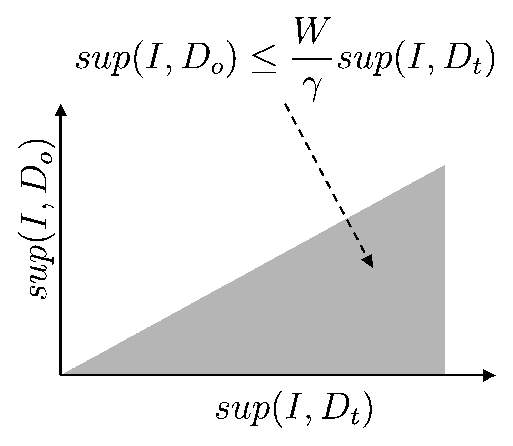
\includegraphics[scale=0.5]{./ep.eps}
\caption{appearance pattern\label{fig:ep}}
\end{center}
\end{minipage}

\begin{minipage}{0.3\hsize}
\begin{center}
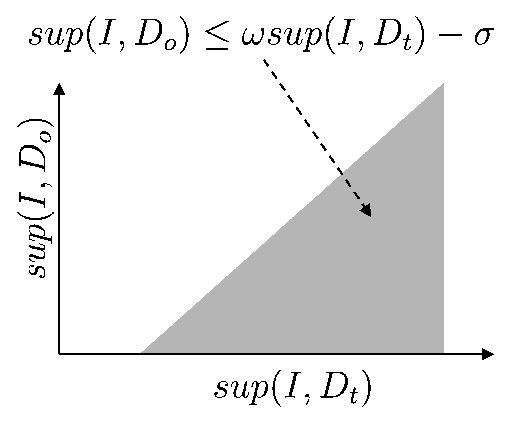
\includegraphics[scale=0.5]{./cp.eps}
\caption{contrast pattern\label{fig:cp}}
\end{center}
\end{minipage}

\begin{minipage}{0.3\hsize}
\begin{center}
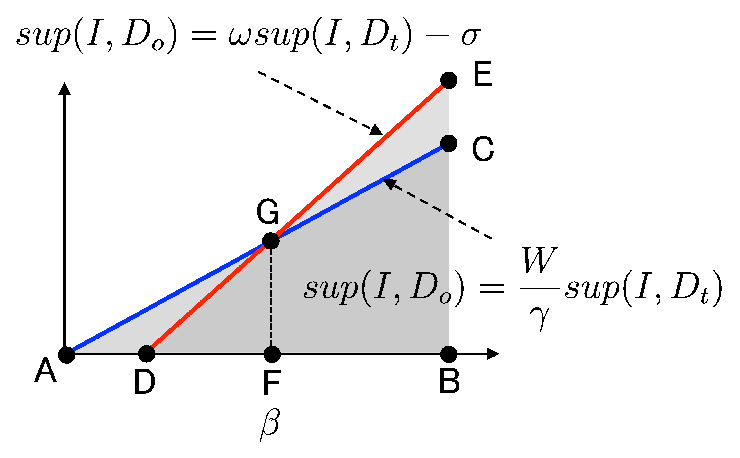
\includegraphics[scale=0.5]{./epcp.eps}
\caption{the relationship between the two patterns\label{fig:epcp}}
\end{center}
\end{minipage}


\end{tabular} 
\end{center}
\end{figure} 

LCM enumerates contrast patterns at high speed based on the parameters $\omega, \sigma$ specified by users.
In enumerating contrast patterns, when $sup(I,D_t)$  becomes larger, sometimes it enumerates patterns with relatively small differences with $sup(I,D_o)$. This pattern is not representative as there is no distinguishable features to class $c_t$.
In order to avoid this drawback, this command uses enumeration of emerging patterns. 

The problem is how to enumerate contrast patterns by using LCM to enumerate emerging patterns. The following illustrates the method adopted for this command.

Diagram \ref{fig:epcp}, \ref{fig:ep} and \ref{fig:cp} are artificially generated.

Instead of enumerating all emerging patterns from area ABC, consider enumerating  emergence pattern from area GFCB which satisfy $sup(I,D_t)\ge\beta$ ($\beta$ is specified at S= parameter in this command).
Patterns enumerated by LCM belongs to $\triangle{DEB}$. The straight line DE is determined by defining $\sigma$ and $\omega$.

Set $\sigma$ as the intersection point G of straight line AC and DE on $x$-coordinate,  and $\beta$ is set  (The method of determining the equation \ref{sigma_beta}):$\omega$ will be discussed below).

By removing $\triangle{DFG}$ and the pattern from $\triangle{EGC}$ from all patterns enumerated from LCM, emerging patterns with distinguish features can be enumerated. 

\begin{equation}
\sigma=\beta (\omega-\frac{W}{\gamma})  \label{sigma_beta}
\end{equation}

Next, find the slope of the line DE corresponding to $\omega$.
In general, the patterns of $\triangle{DGF}$ is far more than the patterns of $\triangle{EGC}$.Thus, it is far more efficient to increase $\omega$.

However, $\omega$ is the weight of transaction, counting on the computer is limited to the maximum value of the variable type.
If the maximum value is $maxInt$, it must satisfy the constraint of $\omega sup(I,D_t)\le maxInt$.

Since $sup(I,D_t)$ will not exceed $|D_p|$, by defining $\omega$ according to the equation (\ref{omega}), the number of enumerations from $\triangle{DFG}$ can be minimised.

\begin{equation}
\omega=\frac{maxInt}{|D_t|} \label{omega}
\end{equation}


